% questions.tex —— 2016 年·全国Ⅱ卷·理科 · 题目内容片段（无答案）
% 由 tools/generate_projects.py 依来源总账自 2016/2016_数学真题_全国2理_试题.md 生成，勿手改（改源 MD 后重跑）


\gkpart{数学}

\begin{gktip}
\textbf{来源说明}：本题面依据固定源 PDF 两页 A3 页面逐题核对，原卷印刷页码 1003–1004。固定源不附答案；本文件仅为题面规范源。
\end{gktip}

\gkpart{一、选择题}

\begin{question}
\gkti{1}已知 \(z=(m+3)+(m-1)i\) 在复平面内对应的点在第四象限，则实数 \(m\) 的取值范围是（　）

   (A) \((-3,1)\)　　(B) \((-1,3)\)　　(C) \((1,+\infty)\)　　(D) \((-\infty,-3)\)

\end{question}
\begin{question}
\gkti{2}已知集合 \(A=\{1,2,3\}\)，\(B=\{x\mid(x+1)(x-2)<0,\ x\in\mathbb Z\}\)，则 \(A\cup B=\)（　）

   (A) \(\{1\}\)　　(B) \(\{1,2\}\)　　(C) \(\{0,1,2,3\}\)　　(D) \(\{-1,0,1,2,3\}\)

\end{question}
\begin{question}
\gkti{3}已知向量 \(\boldsymbol a=(1,m),\ \boldsymbol b=(3,-2)\)，且 \((\boldsymbol a+\boldsymbol b)\perp\boldsymbol b\)，则 \(m=\)（　）

   (A) \(-8\)　　(B) \(-6\)　　(C) \(6\)　　(D) \(8\)

\end{question}
\begin{question}
\gkti{4}圆 \(x^2+y^2-2x-8y+13=0\) 的圆心到直线 \(ax+y-1=0\) 的距离为 1，则 \(a=\)（　）

   (A) \(-\dfrac43\)　　(B) \(-\dfrac34\)　　(C) \(\sqrt3\)　　(D) \(2\)

\Needspace{0.4\textheight}
\end{question}
\begin{question}
\gkti{5}如图，小明从街道的 \(E\) 处出发，先到 \(F\) 处与小红会合，再一起到位于 \(G\) 处的老年公寓参加志愿者活动，则小明到老年公寓可以选择的最短路径条数为（　）
\nopagebreak[4]
\begin{center}% 2016 年全国卷Ⅱ理科第 5 题：街道最短路径图
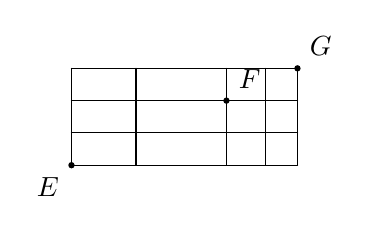
\begin{tikzpicture}[x=0.82cm,y=0.82cm,line cap=round,line join=round]
  % 四列、三行街道网格
  \draw (0,0)--(3.5,0)
        (0,0.5)--(3.5,0.5)
        (0,1.0)--(3.5,1.0)
        (0,1.5)--(3.5,1.5);
  \draw (0,0)--(0,1.5)
        (1.0,0)--(1.0,1.5)
        (2.4,0)--(2.4,1.5)
        (3.0,0)--(3.0,1.5)
        (3.5,0)--(3.5,1.5);
  \fill (0,0) circle (1.15pt);
  \fill (2.4,1.0) circle (1.15pt);
  \fill (3.5,1.5) circle (1.15pt);
  \node[below left=1pt] at (0,0) {$E$};
  \node[above right=1pt] at (2.4,1.0) {$F$};
  \node[above right=1pt] at (3.5,1.5) {$G$};
\end{tikzpicture}
\end{center}
\nopagebreak[4]
   (A) 24　　(B) 18　　(C) 12　　(D) 9

\Needspace{0.4\textheight}
\end{question}
\begin{question}
\gkti{6}如图是由圆柱与圆锥组合而成的几何体的三视图，则该几何体的表面积为（　）
\nopagebreak[4]
\begin{center}% 2016 年全国卷Ⅱ理科第 6 题：圆柱与圆锥组合体的三视图
\begin{tikzpicture}[x=0.55cm,y=0.55cm,>=stealth,line cap=round,line join=round]
  \pgfmathsetmacro{\coneHeight}{2*sqrt(3)}
  % 两个相同的立面轮廓
  \draw (0,0) rectangle (4,4);
  \draw (0,4)--(2,{4+\coneHeight})--(4,4);
  \draw (6,0) rectangle (10,4);
  \draw (6,4)--(8,{4+\coneHeight})--(10,4);

  % 高度尺寸
  \draw[<->] (-0.48,0)--(-0.48,4);
  \draw[<->] (-0.48,4)--(-0.48,{4+\coneHeight});
  \node[left=5pt] at (-0.48,2) {$4$};
  \node[left=5pt] at (-0.48,{4+\coneHeight/2}) {$2\sqrt{3}$};

  % 两个立面底宽尺寸
  \draw (0,0)--(0,-0.48) (4,0)--(4,-0.48);
  \draw[<->] (0,-0.34)--(4,-0.34);
  \node[below=2pt] at (2,-0.34) {$4$};
  \draw (6,0)--(6,-0.48) (10,0)--(10,-0.48);
  \draw[<->] (6,-0.34)--(10,-0.34);
  \node[below=2pt] at (8,-0.34) {$4$};

  % 俯视图及中心点
  \draw (2,-3.3) circle (2);
  \fill (2,-3.3) circle (1.25pt);
\end{tikzpicture}
\end{center}
\nopagebreak[4]
   (A) \(20\pi\)　　(B) \(24\pi\)　　(C) \(28\pi\)　　(D) \(32\pi\)

\end{question}
\begin{question}
\gkti{7}若将函数 \(y=2\sin 2x\) 的图象向左平移 \(\dfrac{\pi}{12}\) 个单位长度，则平移后图象的对称轴为（　）

   (A) \(x=\dfrac{k\pi}{2}-\dfrac{\pi}{6}\ (k\in\mathbb Z)\)　　(B) \(x=\dfrac{k\pi}{2}+\dfrac{\pi}{6}\ (k\in\mathbb Z)\)

   (C) \(x=\dfrac{k\pi}{2}-\dfrac{\pi}{12}\ (k\in\mathbb Z)\)　　(D) \(x=\dfrac{k\pi}{2}+\dfrac{\pi}{12}\ (k\in\mathbb Z)\)

\Needspace{0.4\textheight}
\end{question}
\begin{question}
\gkti{8}中国古代有计算多项式值的秦九韶算法，如图是实现该算法的程序框图。执行该程序框图，若输入的 \(x=2,n=2\)，依次输入的 \(a\) 为 2，2，5，则输出的 \(s=\)（　）
\nopagebreak[4]
\begin{center}% 2016 年全国卷Ⅱ理科第 8 题：秦九韶算法程序框图
\begin{tikzpicture}[>=stealth,line cap=round,line join=round,font=\small]
  % 开始与输入 x,n
  \draw[rounded corners=4pt] (-0.5,6.94) rectangle (0.5,7.36);
  \node at (0,7.15) {开始};
  \draw (-1.0,6.45)--(-0.8,6.0)--(0.8,6.0)--(1.0,6.45)--cycle;
  \node at (0,6.225) {输入 $x,n$};

  % 初始化、输入 a、循环计算
  \draw (-1.1,4.98) rectangle (1.1,5.48);
  \node at (0,5.23) {$k=0,\ s=0$};
  \draw (-0.82,4.47)--(-0.65,3.97)--(0.65,3.97)--(0.82,4.47)--cycle;
  \node at (0,4.22) {输入 $a$};
  \draw (-1.1,2.55) rectangle (1.1,3.35);
  \node at (0,2.95) {\shortstack{$s=s\cdot x+a$\\$k=k+1$}};

  % 判断、输出与结束
  \draw (0,2.25)--(1.3,1.8)--(0,1.35)--(-1.3,1.8)--cycle;
  \node at (0,1.8) {$k>n$};
  \draw (-0.82,0.8)--(-0.65,0.3)--(0.65,0.3)--(0.82,0.8)--cycle;
  \node at (0,0.55) {输出 $s$};
  \draw[rounded corners=4pt] (-0.5,-0.66) rectangle (0.5,-0.24);
  \node at (0,-0.45) {结束};

  % 主流程与“否”分支回到输入 a
  \draw[->] (0,6.94)--(0,6.45);
  \draw[->] (0,6.0)--(0,5.48);
  \draw (0,4.98)--(0,4.72);
  \draw[->] (0,4.72)--(0,4.47);
  \draw[->] (0,3.97)--(0,3.35);
  \draw[->] (0,2.55)--(0,2.2);
  \draw[->] (0,1.4)--(0,0.8);
  \draw[->] (0,0.3)--(0,-0.24);
  \draw (1.3,1.8)--(2.25,1.8)--(2.25,4.72)--(0,4.72);
  \node[right=2pt] at (1.3,2.0) {否};
  \node[right=3pt] at (0,1.08) {是};
\end{tikzpicture}
\end{center}
\nopagebreak[4]
   (A) 7　　(B) 12　　(C) 17　　(D) 34

\end{question}
\begin{question}
\gkti{9}若 \(\cos\left(\dfrac\pi4-\alpha\right)=\dfrac35\)，则 \(\sin 2\alpha=\)（　）

   (A) \(\dfrac7{25}\)　　(B) \(\dfrac15\)　　(C) \(-\dfrac15\)　　(D) \(-\dfrac7{25}\)

\end{question}
\begin{question}
\gkti{10}从区间 \([0,1]\) 随机抽取 \(2n\) 个数 \(x_1,x_2,\cdots,x_n,y_1,y_2,\cdots,y_n\)，构成 \(n\) 个数对 \((x_1,y_1),(x_2,y_2),\cdots,(x_n,y_n)\)，其中两数的平方和小于 1 的数对共有 \(m\) 个，则用随机模拟的方法得到的圆周率的近似值为（　）

   (A) \(\dfrac{4n}{m}\)　　(B) \(\dfrac{2n}{m}\)　　(C) \(\dfrac{4m}{n}\)　　(D) \(\dfrac{2m}{n}\)

\end{question}
\begin{question}
\gkti{11}已知 \(F_1,F_2\) 是双曲线 \(E:\dfrac{x^2}{a^2}-\dfrac{y^2}{b^2}=1\) 的左、右焦点，点 \(M\) 在 \(E\) 上，\(MF_1\) 与 \(x\) 轴垂直，\(\sin\angle MF_2F_1=\dfrac13\)，则 \(E\) 的离心率为（　）

   (A) \(\sqrt2\)　　(B) \(\dfrac32\)　　(C) \(\sqrt3\)　　(D) \(2\)

\end{question}
\begin{question}
\gkti{12}已知函数 \(f(x)\ (x\in\mathbb R)\) 满足 \(f(-x)=2-f(x)\)，若函数 \(y=\dfrac{x+1}{x}\) 与 \(y=f(x)\) 图象的交点为 \((x_1,y_1),(x_2,y_2),\cdots,(x_m,y_m)\)，则 \(\displaystyle\sum_{i=1}^m(x_i+y_i)=\)（　）

   (A) 0　　(B) \(m\)　　(C) \(2m\)　　(D) \(4m\)

\end{question}
\gkpart{二、填空题}

\begin{question}
\gkti{13}\(\triangle ABC\) 的内角 \(A,B,C\) 的对边分别为 \(a,b,c\)，若 \(\cos A=\dfrac45,\ \cos C=\dfrac5{13},\ a=1\)，则 \(b=\underline{\qquad\qquad}\)。

\end{question}
\begin{question}
\gkti{14}\(\alpha,\beta\) 是两个平面，\(m,n\) 是两条线，有下列四个命题：

   ① 如果 \(m\perp n,\ m\perp\alpha,\ n\parallel\beta\)，那么 \(\alpha\perp\beta\)；

   ② 如果 \(m\perp\alpha,\ n\parallel\alpha\)，那么 \(m\perp n\)；

   ③ 如果 \(\alpha\parallel\beta,\ m\subset\alpha\)，那么 \(m\parallel\beta\)；

   ④ 如果 \(m\parallel n,\ \alpha\parallel\beta\)，那么 \(m\) 与 \(\alpha\) 所成的角和 \(n\) 与 \(\beta\) 所成的角相等。

   则上述四个命题中真命题的是\(\underline{\qquad\qquad}\)。

\end{question}
\begin{question}
\gkti{15}有三张卡片，分别写有 1 和 2，1 和 3，2 和 3。甲、乙、丙三人各取走一张卡片，甲看了乙的卡片后说：“我与乙的卡片上相同的数字不是 2”，乙看了丙的卡片后说：“我与丙的卡片上相同的数字不是 1”，丙说：“我的卡片上的数字之和不是 5”，则甲的卡片上的数字是\(\underline{\qquad\qquad}\)。

\end{question}
\begin{question}
\gkti{16}若直线 \(y=kx+b\) 是曲线 \(y=\ln x+2\) 的切线，也是曲线 \(y=\ln(x+1)\) 的切线，\(b=\underline{\qquad\qquad}\)。

\end{question}
\gkpart{三、解答题}

\begin{question}
\gkti{17}\(S_n\) 为等差数列 \(\{a_n\}\) 的前 \(n\) 项和，且 \(a_1=1,\ S_7=28\)。记 \(b_n=\lfloor\lg a_n\rfloor\)，其中 \(\lfloor x\rfloor\) 表示不超过 \(x\) 的最大整数，如 \(\lfloor0.9\rfloor=0,\ \lfloor\lg99\rfloor=1\)。

   (1) 求 \(b_1,b_{11},b_{101}\)；

   (2) 求数列 \(\{b_n\}\) 的前 1000 项和。

\end{question}
\begin{question}
\gkti{18}某险种的基本保费为 \(a\)（单位：元），继续购买该险种的投保人称为续保人，续保人本年度的保费与其上年度出险次数的关联如下：

\begin{center}
\begin{tabular}{lrrrrrr}
\toprule
上年度出险次数 & 0 & 1 & 2 & 3 & 4 & \(\geq5\) \\
\midrule
保费 & \(0.85a\) & \(a\) & \(1.25a\) & \(1.5a\) & \(1.75a\) & \(2a\) \\
\bottomrule
\end{tabular}
\end{center}

设该险种一续保人一年内出险次数与相应概率如下：

\begin{center}
\begin{tabular}{lrrrrrr}
\toprule
一年内出险次数 & 0 & 1 & 2 & 3 & 4 & \(\geq5\) \\
\midrule
概率 & 0.30 & 0.15 & 0.20 & 0.20 & 0.10 & 0.05 \\
\bottomrule
\end{tabular}
\end{center}

   (1) 求一续保人本年度的保费高于基本保费的概率；

   (2) 若一续保人本年度的保费高于基本保费，求其保费比基本保费高出 60\% 的概率；

   (3) 求续保人本年度的平均保费与基本保费的比值。

\Needspace{0.4\textheight}
\end{question}
\begin{question}
\gkti{19}如图，菱形 \(ABCD\) 的对角线 \(AC\) 与 \(BD\) 交于点 \(O\)，\(AB=5,\ AC=6\)，点 \(E,F\) 分别在 \(AD,CD\) 上，\(AE=CF=\dfrac54\)，\(EF\) 交 \(BD\) 于点 \(H\)。将三角形 \(DEF\) 沿 \(EF\) 折到三角形 \(D'EF\) 的位置，\(OD'=\sqrt{10}\)。
\nopagebreak[4]
\begin{center}% 2016 年全国卷Ⅱ理科第 19 题：菱形底面与折起后的 D'
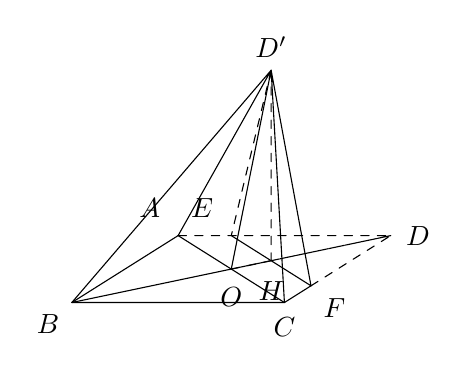
\begin{tikzpicture}[line cap=round,line join=round]
  \coordinate (A)  at (0,1.1);
  \coordinate (B)  at (-1.35,0.25);
  \coordinate (C)  at (1.35,0.25);
  \coordinate (D)  at (2.7,1.1);
  \coordinate (O)  at (0.675,0.675);
  \coordinate (E)  at (0.675,1.1);
  \coordinate (F)  at (1.6875,0.4625);
  \coordinate (H)  at (1.18125,0.78125);
  \coordinate (Dp) at (1.18125,3.2);

  % 按原图保留虚线段，不另作线型含义解释
  \draw[dashed] (A)--(D) (F)--(D) (H)--(D) (Dp)--(H) (Dp)--(E) (O)--(D);

  % 菱形、对角线、折痕与折起后的连线
  \draw (A)--(B)--(C);
  \draw (A)--(C);
  \draw (B)--(H);
  \draw (E)--(F);
  \draw (C)--(F);
  \draw (Dp)--(A) (Dp)--(B) (Dp)--(C) (Dp)--(F) (Dp)--(O);

  \node[above left=3pt] at (A) {$A$};
  \node[below left=1pt] at (B) {$B$};
  \node[below=2pt] at (C) {$C$};
  \node[right=2pt] at (D) {$D$};
  \node[above left=3pt] at (E) {$E$};
  \node[below right=1pt] at (F) {$F$};
  \node[below=3pt] at (O) {$O$};
  \node[below=4pt] at (H) {$H$};
  \node[above=1pt] at (Dp) {$D'$};
\end{tikzpicture}
\end{center}
\nopagebreak[4]
   (1) 证明：\(D'H\perp\) 平面 \(ABCD\)；

   (2) 求二面角 \(B-D'-A-C\) 的正弦值。

\end{question}
\begin{question}
\gkti{20}已知椭圆 \(E:\dfrac{x^2}{t}+\dfrac{y^2}{3}=1\) 的焦点在 \(x\) 轴上，\(A\) 是 \(E\) 的左顶点，斜率为 \(k\ (k>0)\) 的直线交 \(E\) 于 \(A,M\) 两点，点 \(N\) 在 \(E\) 上，\(MA\perp NA\)。

   (1) 当 \(t=4,\ |AM|=|AN|\) 时，求三角形 \(AMN\) 的面积；

   (2) 当 \(2|AM|=|AN|\) 时，求 \(k\) 的取值范围。

\end{question}
\begin{question}
\gkti{21}(1) 讨论函数 \(f(x)=\dfrac{x-2}{x+2}\cdot e^x\) 的单调性，并证明当 \(x>0\) 时，\((x-2)e^x+x+2>0\)；

   (2) 证明：当 \(a\in[0,1)\) 时，函数 \(g(x)=\dfrac{e^x-ax-a}{x^2}\ (x>0)\) 有最小值。设 \(g(x)\) 的最小值为 \(h(a)\)，求函数 \(h(a)\) 的值域。

\Needspace{0.4\textheight}
\end{question}
\begin{question}
\gkti{22}如图，在正方形 \(ABCD\) 中，\(E,G\) 分别在边 \(DA,DC\) 上（不与端点重合），且 \(DE=DG\)，过 \(D\) 点作 \(DF\perp CE\)，垂足为 \(F\)。
\nopagebreak[4]
\begin{center}% 2016 年全国卷Ⅱ理科第 22 题：正方形内的垂足与连线
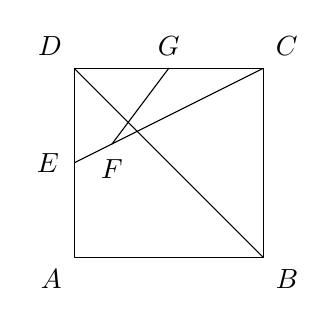
\begin{tikzpicture}[line cap=round,line join=round]
  \coordinate (A) at (0,0);
  \coordinate (B) at (2.4,0);
  \coordinate (C) at (2.4,2.4);
  \coordinate (D) at (0,2.4);
  \coordinate (E) at (0,1.2);
  \coordinate (G) at (1.2,2.4);
  \coordinate (F) at (0.48,1.44);

  \draw (A)--(B)--(C)--(D)--cycle;
  \draw (D)--(B);
  \draw (E)--(C);
  \draw (F)--(G);

  \node[below left=1pt] at (A) {$A$};
  \node[below right=1pt] at (B) {$B$};
  \node[above right=1pt] at (C) {$C$};
  \node[above left=1pt] at (D) {$D$};
  \node[left=2pt] at (E) {$E$};
  \node[above=1pt] at (G) {$G$};
  \node[below=2pt] at (F) {$F$};
\end{tikzpicture}
\end{center}
\nopagebreak[4]
   (1) 证明：\(B,C,G,F\) 四点共圆；

   (2) 若 \(AB=1,\ E\) 为 \(DA\) 的中点，求四边形 \(BCGF\) 的面积。

\end{question}
\begin{question}
\gkti{23}在直角坐标系 \(xOy\) 中，圆 \(C\) 的方程为 \((x+6)^2+y^2=25\)。

   (1) 以坐标原点为极点，\(x\) 轴正半轴为极轴建立极坐标系，求圆 \(C\) 的极坐标方程；

   (2) 直线 \(l\) 的参数方程是 \(\begin{cases}x=t\cos\alpha,\\y=t\sin\alpha,\end{cases}\)（\(t\) 为参数），直线 \(l\) 与圆 \(C\) 交于 \(A,B\) 两点，\(|AB|=\sqrt{10}\)，求 \(l\) 的斜率。

\end{question}
\begin{question}
\gkti{24}已知函数 \(f(x)=\left|x-\dfrac12\right|+\left|x+\dfrac12\right|\)，\(M\) 为不等式 \(f(x)<2\) 的解集。

   (1) 求 \(M\)；

   (2) 证明：当 \(a,b\in M\) 时，\(|a+b|<|1+ab|\)。

\end{question}